\documentclass[../bccalc.tex]{subfiles}
\graphicspath{{\subfix{../figures/}}}
\begin{document}
\chapter{Applications of Differentiation}
\section{Definition of the Derivative Meets Derivative Rules}
\begin{example}
    Evaluate the following by recognizing that the given limit represents a derivative. 
    \[ \lim_{h\to 0} \frac{2(x+h)^3-2x^3}{h} \]

    We know $f(x)=2x^3$, so the derivative is trivial from this.
\end{example}

\ex Evaluate the following by recognizing the given limit represents a derivative. 

$\lim_{h\to 0} \frac{\cos (5(x+h)) - \cos(5x)}{h}$

\ex Evaluate the following by recognizing the given limit represents a derivative. 

$\lim_{h\to 0} \frac{\sin \left(\frac{\pi}{6}+h\right)-\frac{1}{2}}{h}$

\section{Related Rates}
We have previously learned the Chain Rule and this allows us to use implicit differentiation for related rates.

\begin{example}
    Suppose $y=5x^2-6x+2$. Find $\frac{dy}{dt}$ when $x=4$, given that $\frac{dx}{dt}=2$ when $x=4$.

    We are taking the derivative of $y$ with respect to $t$.

    We get $\frac{dy}{dt}(y=5x^2-6x+2)=\frac{dy}{dt}=10x\frac{dx}{dt}-6\frac{dx}{dt}$.

    Plug this in to get $68$ as the answer.
\end{example}

\begin{example}
    A pebble is dropped into a calm pond, causing ripples in the shape of concentric circles. The radius of the outer ripple is increasing at a constant rate of 1 ft/sec. When the radius is 4 ft, find the rate at which the area of the disturbed water is changing.

    We have to do the derivative of $A=\pi r^2$, the circle formula.

    This is $2\pi r \frac{dr}{dt}$. Plug in numbers to get $8 \pi$ ft$^2$/sec
\end{example}

\ex Water runs out of a conical tank at the constant rate of 2 cubic feet per minute. The radius at the top of the tank is 5 feet, and the height of the tank is 10 feet. How fast is the water level sinking when the water is 4 feet deep?
\pagebreak
\begin{example}
    A fish is reeled in at a rate of 2 ft/sec from a bridge 16 ft above the water. At what rate is the angle between the line and the water changing when there are 20 ft of line out?

    If we let $x$ be the distance from the fish to the person, then we know $\frac{dx}{dt} = -2$.

    We are trying to find $\frac{d\theta}{dt}$.

    Using trig, we can find $\tan \theta = 16x^{-1}$.

    The derivative gives $\sec^2 \theta\frac{d\theta}{dt}=-16x^{-2}\frac{dx}{dt}$.

    Plugging in numbers and solving for $\frac{d\theta}{dt}=\frac{2}{25}$ rad/s.
\end{example}

\ex A man 6 ft tall walks at a rate of 5 ft/sec away from a lightpole 16 ft tall. 

(a) At what rate is the tip of his shadow moving when he is 10 ft from the base of the light?

(b) At what rate is the length of his shadow moving when he is 10 ft from the base of the light?

\ex A trough is 10 ft long and 6 ft across the top. Its ends are isosceles triangles with an altitude of 4 ft. If water is being pumped into the trough at 9 ft$^3$/sec, how fast is the water level rising when the water is 2 ft deep?

\section{Extrema on an Interval}
\begin{definition}[Definition of Extrema]
    Let $f$ be defined on an interval $I$ containing $c$.
    \begin{enumerate}
        \item $f(c)$ is the minimum of $f$ on $I$ if $f(c)\leq f(x)$ for all $x$ in $I$.
        \item $f(c)$ is the maximum of $f$ on $I$ if $f(c)\geq f(x)$ for all $x$ in $I$.
    \end{enumerate}

    The minimum and maximum of a function on an interval are the extreme values or extrema of the function on the interval. The minimum and maximum of a function on an interval are also called the absolute minimum and absolute maximum, or the global minimum and global maximum, on the interval.
\end{definition}

\begin{definition}[Relative Extrema]
    \begin{enumerate}
        \item If there is an open interval containing $c$ on which $f(c)$ is a maximum, then $(c, f(c))$ is called a relative maximum of $f$, or you can say that $f$ has a relative maximum at $(c,f(c))$.
        \item If there is an open interval containing $c$ on which $f(c)$ is a minimum, then $(c,f(c))$ is called a relative minimum on $f$, or you can say that $f$ has a relative minimum at $(c,f(c))$.
    \end{enumerate}

    The relative maximum and relative minimum points are sometimes called local maximum and local minimum points, respectively.
\end{definition}
\pagebreak
\begin{example}
    In the figure, wind where $f$ has an absolute maximum, absolute minimum, relative maximum, and relative minimum on the interval $[-2,4]$.
    \begin{center}
        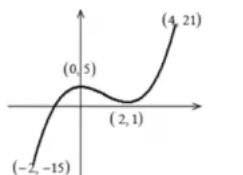
\includegraphics[width=0.3\textwidth]{3.1.1.PNG}
    \end{center}
    Absolute maximum at 4, absolute minimum at $-2$, relative maximum at 0, relative minimum at 2.
\end{example}

\begin{definition}[Critical Number and Critical Point]
    Let $f$ be defined at $c$. If $f'(c)=0$ or if $f$ is not differentiable at $c$, then $c$ is a critical number of $f$ and the point $(c,f(c))$ is a critical opint of $f$.
\end{definition}

\begin{theorem}
    Relative extrama occur only at critical numbers.
\end{theorem}

\begin{example}
    In the following, name the maximum and minimum points.
    \begin{center}
        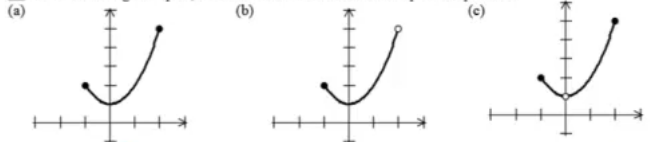
\includegraphics[width=0.7\textwidth]{3.1.2.png}
    \end{center}

    (a) Minimum at 0, maximum at 2 

    (b) Minimum at 0, no maximum 

    (c) no minimum, maximum at 2
\end{example}

Continuity is needed to guarantee a maximum and minimum.

\begin{theorem}[Extreme Value Theorem]
    If $f$ is continuous on a closed interval $[a,b]$, then $f$ attains an absolute maximum value $f(c)$ or an absolute minimum value $f(d)$ for some numbers $c$ and $d$ in $[a,b]$.
\end{theorem}

Guidelines for Finding Extrema on a Closed Interval - Candidates Test 

To find the extrema of a continuous function $f$ on a closed interval $[a,b]$, we used the following steps:
\begin{enumerate}
    \item Find $f'(x)$ and the critical numbers of $f$ in $[a,b]$.
    \item Evaluate $f$ at each critical number in $(a,b)$.
    \item Evaluate $f$ at each endpoint in $[a,b]$.
    \item The least of these values is the minimum. The greatest is the maximum.
\end{enumerate}

\begin{example}
    Find the absolute maximums and minimums of $f$ on the given closed interval, and state where these values occur.

    (a) $f(x)=3x^2-24x-1 \qquad [-1,5]$

    $f'(x)=0$ when $x=4$.

    $f$ has an absolute maximum of 26 at $x=-1$ and $f$ has an absolute minimum of $-49$ at $x=4$.

    (b) $f(x)=6x^3-6x^4+5 \qquad [-1,2]$.

    $f'(x)=18x^2-24x^3=0$.

    $x=0$ and $x=3/4$.

    $f$ has an absolute maximum of 5.6328 at $x=3/4$ and an absolute minimum of $-43$ at $x=2$.
\end{example}

\ex Same as above for $f(x)=3x^{2/3}-2x+1 \qquad [-1,8]$

\ex Same as above for $f(x)=\sin^2 x+\cos x\qquad [0,2\pi]$



\section{Mean Value Theorem and Rolle's Theorem}
\begin{theorem}[Mean Value Theorem]
    If a function $f$ is: 

    \begin{enumerate}
        \item continuous on $[a,b]$ and 
        \item differentiable on $(a,b)$
    \end{enumerate}
    then there is at least one number $c$ in $(a,b)$ such that 
    \begin{enumerate}
        \item $\frac{f(b)-f(a)}{b-a}=f'(c)$
        \item $f(b)-f(a)=f'(c)(b-a)$
        \item $f(b)=f(a)+f'(c)(b-a)$
    \end{enumerate}
\end{theorem}

If $f(a)$ and $f(b)$ are equal, this special case of the Mean Value Theorem is called Rolle's Theorem.
\begin{theorem}[Rolle's Theorem]
    If a function $f$ is 
    \begin{enumerate}
        \item continuous on $[a,b]$ and 
        \item differentiable on $(a,b)$ and 
        \item $f(a)=f(b)$
    \end{enumerate}
    then there is at least one number $c$ in $(a,b)$ such that 
    \begin{enumerate}
        \item $\frac{f(b)-f(a)}{b-a}=f'(c)$
        \item $\frac{0}{b-a}=f'(c)$
        \item $0=f'(c)$
    \end{enumerate}
\end{theorem}
\pagebreak
\begin{example}
    Show that the conditions of Rolle's Theorem are met, and find the $c$ that Rolle's Theorem guarantees.

    \[ f(x)=x^2-x-6 \quad [-2,3] \]

    This is a continuous and differentiable function.

    $f(3)=0$ and $f(-2)=0$, so $f'(x)=2x-1=0$, so $x=1/2$.
\end{example}

\ex Given the function $f(x)=3-\frac{5}{x}$ on the interval $[1,5]$, show that the Mean Value Theorem applies, and find the $c$ that the theorem guarantees.

\begin{example}
    You are driving a car traveling on an interstate at 50 mph, and you pass a police car. Four minutes later, you pass a second police car, and you are again traveling at 50 mph.
    The speed limit on the interstate is 60 mph. The distance between the two police cars is five miles. The patrolman in the second police car gives you a speeding ticket for driving 75 mph. How can he prove that you were speeding?

    $r=\frac{d}{t}=75$ mph. Since speed is a differnetiable function of time and averaged 75 mph, the MVT says there is at least one time in those 4 minutes where the instantaneous rate of change is 75 mph.
\end{example}

\section{Increasing and Decreasing Functions and the First Derivative Test}
\begin{definition}
    \begin{enumerate}
        \item A function $f$ is increasing on an interval if for any two numbers 
        
        $x_1$ and $x_2$ in the interval, $x_1<x_2$ implies $f(x_1)<f(x_2)$.

        \item A function $f$ is decreasing on an interval if for any two numbers 
        
        $x_1$ and $x_2$ in the interval, $x_1<x_2$ implies $f(x_1)>f(x_2)$
    \end{enumerate}
\end{definition}

Test for Increasing and Decreasing Functions 
\begin{enumerate}
    \item If $f'(x)>0$ for all $x$ in $(a,b)$, then $f$ is increasing on $[a,b]$.
    \item If $f'(x)<0$ for all $x$ in $(a,b)$, then $f$ is decreasing on $[a,b]$.
    \item If $f'(x)=0$ for all $x$ in $(a,b)$, then $f$ is constant on $[a,b]$.
\end{enumerate}

First Derivative Test:

Let $c$ be a critical number of a function $f$ that is continuous on an open interval $I$ containing $c$. If $f$ is differentiable on the interval, except possibly at $c$, then $(c,f(c))$ can be classified as follows.
\begin{enumerate}
    \item If $f'(x)$ changes from negative to positive at $x=c$, then $(c,f(c))$ is a relative minimum of $f$.
    \item If $f'(x)$ changes from positive to negative at $x=c$, then $(c,f(c))$ is a relative maximum of $f$.
\end{enumerate}
\pagebreak
\begin{example}
    Find the intervals where $f$ is increasing and decreasing, identify all points that are relative maximum and minimum points, and justify your answers.

    \[ f(x)=\frac{1}{3}x^3-x^2-3x+2 \]

    $f'(x)=x^2-2x-3$ or $(x-3)(x+1)=0$.

    We can try points, $f'(-2)=5$, $f'(0)=-3$, $f'(4)=5$.

    $f$ is increasing on $(-\infty]\cup [3,\infty)$ because $f'$ is positive and decreasing on $[-1,3]$ because $f'$ is negative.

    $f$ has a relative maximum at $-1$ because $f'$ changes from positive to negative.

    $f$ has a relative minimum at $x=3$ because $f'$ changes from negative to positive.    
\end{example}

\ex Do the same as above for the function $f(x)=(x^2-4)^{2/3}$

\ex Do the same above for the function $f(x)=\frac{x^2}{2x-1}$

\ex Do the same above for the function $f(x)=\begin{cases}
    2x+1, & x\leq -1 \\
    x^2-2, & x>-1
\end{cases}$

\begin{example}
    Use the graph of $f'$ to: 

    (a) identify the interval(s) on which the graph of $f$ is increasing and decreasing 

    (b) estimate the value(s) of $x$ at which the graph of $f$ has a relative maximum or minimum. Justify your answers.

    \begin{center}
        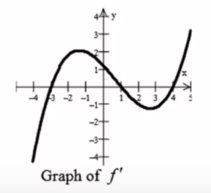
\includegraphics[width=0.3\textwidth]{3.2.1.png}
    \end{center}

    We can see critial points are $-3,1,4$ when they cross the $x$-axis.

    Looking at the graph, $(-3,1)\cup (4,\infty)$ $f$ is increasing on this interval because $f'>0$ and $f$ has a relative maximum at $x=1$ because $f'$ goes positive to negative.

    From the interval $(-\infty,-3)\cup (1,4)$ $f$ is decreasing because $f'<0$ and $f$ has a relative minimum at $-3$ and $4$ because $f'$ goes negative to positive. 
\end{example}

\ex Given $f'(x)<0$ on $(-\infty,3)$, $f'(x)>0$ on $(-3,2)$, $f'(x)<0$ on $(2,\infty)$. 

(a) If $g(x)=2f(x)$, what is the sign of $g'(-1)$?

(b) If $g(x)=f(3x-5)$, what is the sign of $g'(-1)$?

\pagebreak
\begin{example}
    The function $s(t)=t^2-7t+10$ describes the motion of a particle along a line.

(a) Find the velocity function of the particle at any time $t\geq 0$.

$v(t)=2t-7$

(b) Identify the time interval(s) in which the particle is moving in a positive direction. Justify.

$(7/2,\infty)$ because $v(t)=s'(t)>0$

(c) Identify the interval(s) in which the particle is moving in a negative direction. Justify.

$(-\infty,7/2)$ because $v(t)=s'(t)<0$

(d) Identify the time(s) at which the particle changes direction. Justify.

$t=7/2$ because $v(t)$ changes from negative to positive.
\end{example}


\section{Concavity and the Second Derivative}
\begin{definition}[Concavity]
    Let $f$ be differentiable on an open interval $I$.

    \begin{enumerate}
        \item The graph of $f$ is concave upward on an interval $I$ if $f'$ is increasing on the interval.
        \item The graph of $f$ is concave downward on an interval $I$ if $f'$ is decreasing on the interval.
    \end{enumerate}
\end{definition}

Test for Concavity
\begin{enumerate}
    \item If $f''(x)>0$ for all $x$ in $I$, then the graph of $f$ is concave up in $I$.
    \item If $f''(x)<0$ for all $x$ in $I$, then the graph of $f$ is concave down in $I$.
\end{enumerate}

\begin{definition}[Inflection Point]
    A function $f$ has an inflection point at $(c,f(c))$

    \begin{enumerate}
        \item if $f''=0$ or if $f''$ does not exist and 
        \item if $f''$ changes sign from negative to positive or positive to negative at $x=c$ OR if $f'(x)$ changes from increasing to decreasing or decreasing to increasing at $x=c$.
    \end{enumerate}
\end{definition}

\begin{example}
    The graph of $f$ is shown below. State the signs of $f'$ and $f''$ on the interval $(0,3)$.
    \begin{center}
        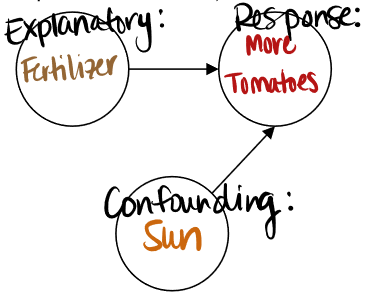
\includegraphics[width=0.3\textwidth]{3.3.1.PNG}
    \end{center}

    $f$ is decreasing the whole time, so $f'<0$, but $f'$ is increasing so $f''>0$.
\end{example}

\begin{example}
    Given the function $f(x)=x^4-4x^3$ find:

    (a) the intervals where $f$ is increasing and decreasing 

    $f$ is decreasing on $(-\infty,0)\cup (0,3)$ because $f'<0$.

    $f$ is increasing on $(3,\infty)$ because $f'>0$.

    (b) the relative extrema 

    $f$ has a relative minimum at $x=3$ because $f'$ changes negative to positive.

    (c) the intervals where $f$ is concave up and concave down 

    Concave up: $(-\infty,0)\cup (2,\infty)$.

    Concave down: $(0,2)$

    (d) the inflection points 

    $x=0$ and $x=2$
\end{example}

\ex Sketch a graph for the following characteristics

(a)
\begin{itemize}
    \item $f(0)=f(2)=0$
    \item $f'(x)>0$ if $x<1$
    \item $f'(1)=0$
    \item $f'(x)<0$ if $x>1$
    \item $f''(x)<0$
\end{itemize}

(b)
\begin{itemize}
    \item $f(0)=f(2)=0$
    \item $f'(x)>0$ if $x<1$
    \item $f'(1)$ is undefined 
    \item $f'(x)<0$ if $x>1$
    \item $f''(x)>0$
\end{itemize}


\section{Second Derivative Test}
Second Derivative Test:

Let $f$ be a function such that the second derivative of $f$ exists on an open interval containing $c$.
\begin{enumerate}
    \item If $f'(c)=0$ and $f''(c)>0$, then $f(c)$ is a relative minimum of $f$.
    \item If $f'(c)=0$ and $f''(c)<0$, then $f(c)$ is a relative maximum of $f$.
\end{enumerate}
\pagebreak
\begin{example}
    Use the Second Derivative Test, if possible, to find the relative extrema of $f(x)=-3x^5+5x^3$. Justify your answer.

    The first derivative is $-15x^4+15x^2$. We can factor this to get $x=0,\pm 1$.

    $f''(x)=-60x^3+30x$, $f''(1)=-30<0$, $f''(-1)=30>0$ and $f''(0)=0$.

    So we can see there is a relative maximum at $x=1$ because $f'=0$ and $f''<0$.

    There is a relative minimum at $x=-1$ because $f'=0$ and $f''>0$.
\end{example}

\ex Suppose that the function $f$ has a continuous second derivative for all $x$, and that $f(3)=-4, f'(3)=1, f''(3)=-2$. Let $g$ be a function whose derivative is given by $g'(x)=(x^2-9)(2f(x)+5f'(x))$ for all $x$. Does $g$ have a local maximum or a local minimum at $x=3$. Justify your answer.

\section{Graphs of f, f', and f''}
\begin{example}
    \begin{center}
        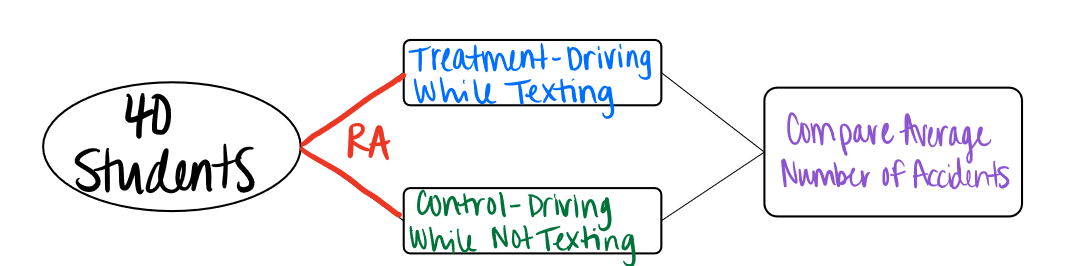
\includegraphics[width=0.3\textwidth]{3.4.1.PNG}
    \end{center}
    The graph of $y=f'(x)$ is given above. The domain of $f$ is $[-3,3]$.

    (a) For what value(s) of $x, -3<x<3$, is the graph of $f$ increasing? Justify your answer.

    $(-3,-2)\cup (0,2)\cup (2,3)$ because $f'>0$.

    (b) For what value(s) of $x,-3<x<3$, does the graph of $f$ have a relative maximum? Justify your answer.

    $f$ has a relative maximum at $x=-2$ because $f'$ goes from positive to negative.

    (c) For what value(s) of $x, -3<x<3$, is the graph of $f$ concave down? Justify your answer.

    $f$ is concave down on $(-3,-1)\cup (1,2)$ because $f$ is decreasing.

    (d) For what value(s) of $x,-3<x<3$, does the graph of $f$ have an inflection point? Justify your answer.

    $f$ has a point of inflection at $x=-1,1,2$ because $f'$ changes from decreasing to increasing at this point.
\end{example}
\ex Using the information above, and the fact that $f(-3)=0$ sketch a possible graph for $f$.

\end{document}